\chapter{Introducción}
\noindent
La administración de redes se dedica a establecer las actividades que deben realizarse sobre una red informática con el fin de brindar los diferentes servicios de manera eficiente y eficaz, garantizando la disponibilidad y calidad que el usuario final espera. En la administración de redes es muy usado el protocolo SNMP o protocolo simple de Administración de red, que facilita el intercambio de paquetes de información de administración entre los diferentes dispositivos de la red. La administración de las redes, también consiste en tener un constante monitoreo de como se comportan las mismas, esto con la finalidad de poder prevenir malos funcionamientos y en caso de que estos se presentasen, poder actuar de forma correcta. La administración de fallos, es una parte fundamental de la administración de servicios, algunos conceptos básicos son presentados a continuación.

\section{FCAPS}
FCAPS es un marco de gestión de redes que fue creado por la Organización Internacional de Normalización, mejor conocida como  ISO (por sus siglas en inglés).
\newline
Las siglas FCAPS significan:
\begin{itemize}
    \item F (Fault): Fallas.
    \item C (Configuration): Configuración.
    \item A (Accounting): Administración.
    \item P (Performance): Desempeño.
    \item S (Security): Seguridad.
\end{itemize}

En esta práctica, nos enfocaremos en la F, es decir la Administración de Fallas.
\newline
Una falla, se puede definir como un evento que muestra un problema en la red. El objetivo de la administración de fallas es el de detectar, aislar, corregir y registrar fallas que ocurren en la red. 
\newline
La administración de fallas también incluye el análisis de tendencias para predecir errores, de modo que la red siempre brinde el servicio que pretende o para lo que fue diseñada.
\newline
Para gestionar las fallas, se requiere de un sistema para monitorear la red y que pueda generar alarmas o notificaciones. Un sistema básico de gestión de alarmas proporciona una lista de alarmas basadas en la topología de la red. Una vez que se activan las alarmas o los usuarios de la red enfrentan un problema, se requiere un sistema de tickets para administrar la carga de trabajo y las prioridades asociadas con las fallas. 
\newline
Una alarma solo muestra el síntoma de un problema, por lo que adicionalmente, se requiere de un sistema que brinde la solución de problemas para recopilar más información sobre las posibles causas que llevan a la falla \cite{FCAPS}.

\section{Línea base}
Una línea de base o línea de fondo, consiste en un proceso que permite estudiar la red con base en intervalos regulares, esto con el objetivo de asegurarse de que la red se encuentra trabajando acorde a lo que fue diseñada.
\newline
La línea de base sirve para obtener información de importancia como:
\begin{itemize}
    \item Información de la salud del hardware y software de la red
    \item Determinar los usos de los recursos de la red
    \item Tomar decisiones precisas sobre los umbrales de alarmas de la red
    \item Identificar los problemas o fallas de la red
    \item Predecir problemas o fallas futuros
\end{itemize}
A grandes rasgos, consiste en definir un umbral, o bien 3 (Ready, Set, Go), a partir de los cuales en el momento en que el estado actual de la red graficada cruce las líneas previamente definidias, se identificará como una falla \cite{LineaBase}.
\begin{figure}[H]
\vspace{1cm}
\centering
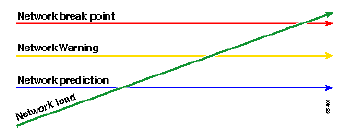
\includegraphics[width=0.6\textwidth]{imagenes/lineaBase.PNG}
\caption{Representación gráfica de línea base}
\end{figure}

\section{Mínimos cuadrados}
El método de mínimos cuadrados permite obtener una línea del mejor ajuste de forma más precisa.
\newline
Los pasos para este método son \cite{MinimosCuadrados}:
\begin{itemize}
    \item Calcular la media de los valores x así como la media de los valores y
    \item Calcular la pendiente de la línea de mejor ajuste
    \item Calcular la intercepción en y de la línea usando la fórmula de la recta.
    \item Utilizar la pendiente m y la intercepción en y para formar la ecuación de la recta.
\end{itemize}
\begin{figure}[H]
\vspace{1cm}
\centering
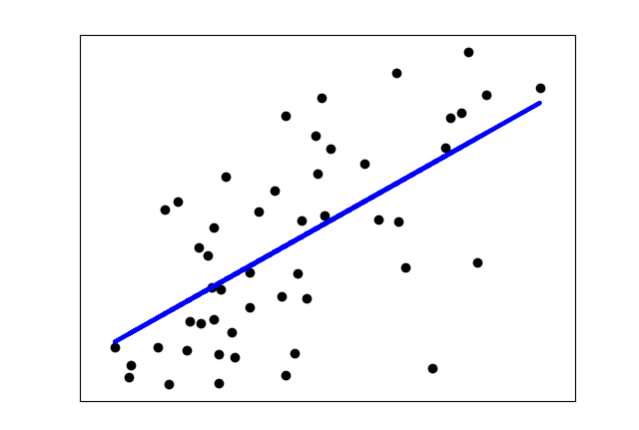
\includegraphics[width=0.8\textwidth]{imagenes/minimoscuadrados.png}
\caption{Representación gráfica de mínimos cuadrados}
\end{figure}

\section{Holt Winters}
El método de Holt-Winters cocnsiste en un método que ofrece un pronóstico de triple exponente suavizante. Este método tiene la ventaja de poder adaptarse con mayor facilidad a medida que obtiene nueva información real. 
\newline
Este método considera nivel, tendencia y estacional de una determinada serie de tiempos.
\newline
Holt-Winters se aplica solamente cuando la serie de datos es estacional, es decir, es periódica. 
\newline
Por medio de este método se puede detectar y hacer predicciones de comportamiento anómalo\cite{HoltWinters}. 
\newline
Dos conceptos muy importantes para Holt-Winters son:
\begin{itemize}
    \item Valor observado: Se trata de aquellos valores que ya conocemos.
    \item Valor esperado: Se trata de aquellos valores que resultan de una predicción con base a los valores observados.
\end{itemize}

\begin{figure}[H]
\vspace{1cm}
\centering
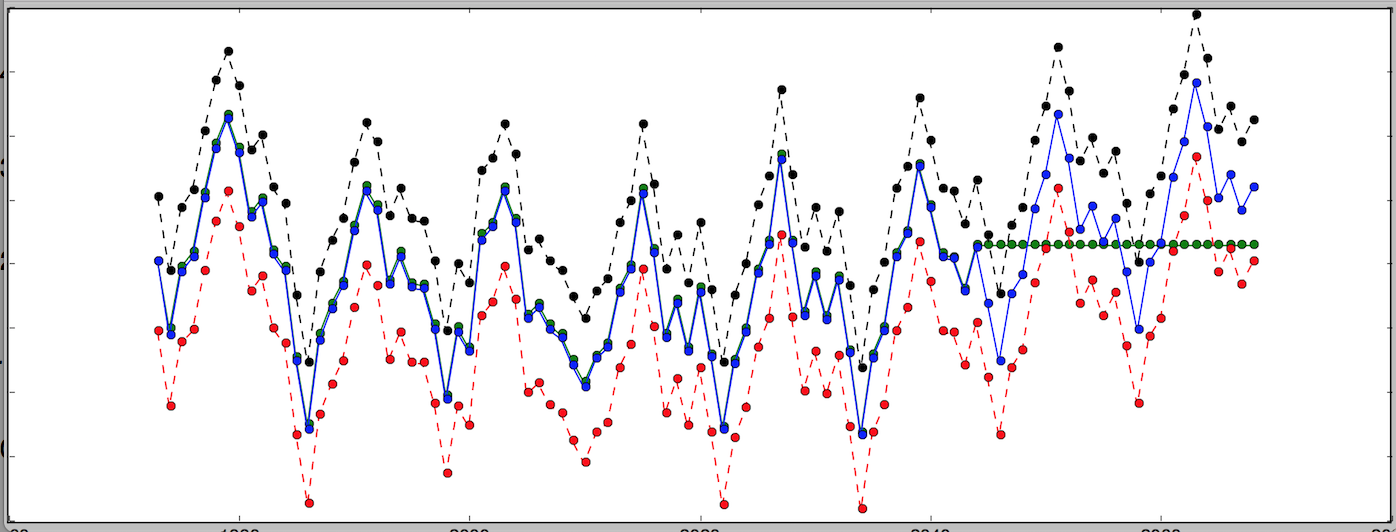
\includegraphics[width=0.8\textwidth]{imagenes/hw.png}
\caption{Representación gráfica de Holt Winters}
\end{figure}